\chapter{Implementação} \label{cap:implementacao}

Para facilitar a manutenção e implementação do sistema, bem como a sua compreesão,o \textbf{SecDash} encontra-se decomposto em camadas, seguindo um padrão de desenho \textit{multi-tier} ou \textit{layered}. \\

A aplicação encontra-se dividida em três níveis, numa estrutura hierárquica, sendo estes a \textbf{camada de apresentação}, a \textbf{camada lógica} e a \textbf{camada de dados}. \\

\begin{itemize}
	\item A \textbf{camada de apresentação} tem como função principal ser a interface com a qual o utilizador interage com o \textbf{SecDash}, isto é, o nosso \textit{frontend} web;

	\item A \textbf{camada lógica} é o cerne do programa, tratando-se do nosso backend em kotlin onde é implementada toda a lógica de negócio;

	\item A \textbf{camada de dados} persiste os dados a serem armazenados permanentemente, estando esta implementada como uma base de dados PostgreSQL; 
\end{itemize}

Os detalhes e especifidades da implementação e desenvolvimeto de cada uma destas camadas serão explorados ao longo deste capítulo. \\

\section{Modelo de dados} \label{implementacao:modelo}
A elaboração de um modelo Entidade-Associação é indispensável para a estruturação lógica do projeto. Com efeito, é a existência de um modelo entidade-associação que permite estruturar de forma concreta as entidades do domínio da aplicação e as suas relações entre si. \\

O modelo de dados serve também de ponte entre os requisitos de negócio da plataforma e a sua implementação física na base de dados. Este mapeamento garante que a existência uma visão clara de como os utilizadores, repositórios e vulnerabilidades se relacionam entre si, permitindo orientar a implementação lógica do sistema prevenindo assim o aparecimento de inconsistências estruturais que pudessem pôr em causa a robustez da aplicação ou atrasar o seu desenvolvimento. \\

Como referido no capítulo anterior, os dados obtidos das APIs externas do GitHub e GitLab são altamente estruturados e com dependências e relações claras entre si. Assim sendo, a elaboração de um modelo Entidade-Associação, indispensável para a estruturação lógica do projeto, torna-se relativamente trivial. \\

O diagrama do modelo obtido encontra-se apresentado na figura abaixo. É importante salientar que, de forma a facilitar a apresentação e visualização do modelo no presente documento, os atributos das entidades, bem como a cardinalidade das suas relações, foram omitidos do diagrama. O script SQL utilizado para criar todo o esquema da base de dados, onde se pode consultar todos os atributos, encontra-se no Apêndice \ref{ap:schema}. \\

\begin{figure}[h]
	\centering
	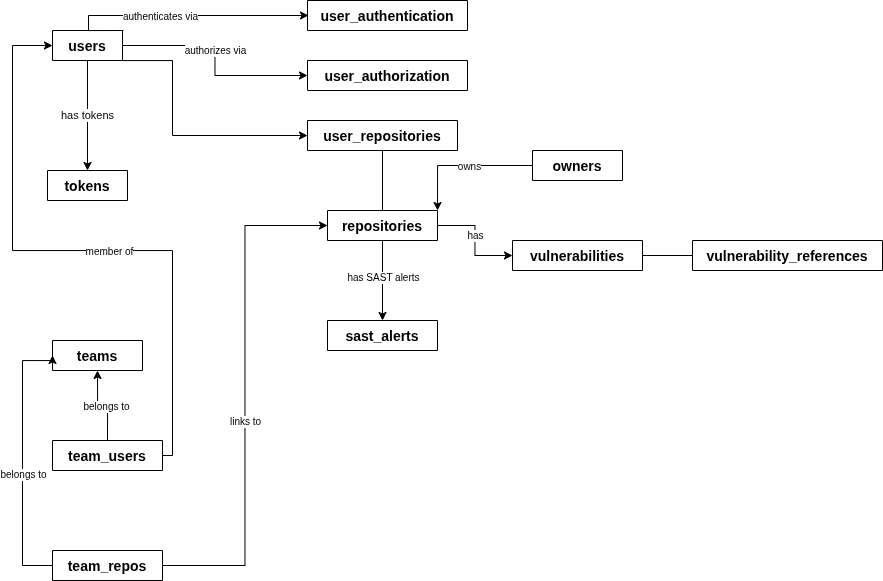
\includegraphics[width=0.95\linewidth]{./figures/secdash-ea.drawio.png}
	\caption{diagrama do modelo de dados}
\end{figure}

\begin{itemize}
	\item Cada \textbf{USER} possui um \textbf{id} que os identificará na aplicação, bem como um \textbf{name} e \textbf{email}. Poderão também ter um campo \textit{\textbf{password\_validation}}, opcional, caso optem por se registar na aplicação diretamente com o seu email em vez de utilizarem uma das opções OAuth 2.0. \\
	
	Cada user terá também uma \textit{\textbf{role}}, que o identificará como um utilizador normal ou administrador, tendo este último acesso a funcionalidades vedadas a utilizadores normais, tais como eliminar utilizadores ou equipas que não lhe pertencem. \\
	
	As informações de autenticação são guardadas na tabela \textbf{USER\_AUTHENTICATION}, que irá conter os IDs de cada utilizador, o provedor de autenticação OAuth 2.0  (Google, GitHub ou GitLab) e o ID do utilizador nessa plataforma. \\
	
 	Os \textit{access tokens} de cada utilizador ficam armazenados na tabela \textbf{USER\_AUTHORIZATION}. Os \textit{tokens} internos gerados e usados pelo próprio \textbf{SecDash}, por sua vez, são armazedados na tabela \textbf{TOKENS}. \\
	
	\item Cada repositório vigiado pela aplicação é armazenado na tabela \textbf{REPOSITORIES}. A tabela \textbf{OWNERS} armazena algumas informações referentes aos proprietários dos repositórios nas plataformas de origem, seja ela GitHub ou GitLab. Para fazer a ligação entre os repositórios armazenados e os utilizadores que os vigiam existe a tabela \textbf{USER\_REPOSITORIES}. \\ 
	
	Os alertas SAST e vulnerabilidades detetadas nas dependências de cada repositório são armazenados nas tabelas \textbf{SAST\_ALERTS} e \textbf{VULNERABILITIES} respetivamente. Esta última tabela encontra-se também ligada à tabela \textbf{VULNERABILITY\_REFERENCES}, que armazena ligações as CVEs onde essas vulnerabilidades estão catalogadas. \\
	
	\item Finalmente, as informações de cada equipa criada no âmbito da aplicação são armazenadas da tabela \textbf{TEAMS}. Os repositórios e utilizadores ligados a cada uma são armazenados nas tabelas \textbf{TEAM\_REPOS} e \textbf{TEAM\_USERS} respetivamente. \\
\end{itemize}

É importante indicar que ao obter os dados das APIs externas, sejam estes referentes a repositórios ou vulnerabilidades, a informação devolvida contém inúmeros campos que não consideramos relevantes de armazenar ou exibir aos utilizadores para os propósitos do \textbf{SecDash}. A título de exemplo, o objeto JSON referente a um repoisitório GitHub devolvido pela sua API contém mais de 80 campos, sendo vários deles objetos que por sua vez contém também múltiplos campos. Um exemplo deste formato pode ser consultado no Apêndice \ref{ap:repogithub}. Como tal, optou-se por filtrar muitos destes campos, sendo apenas armazenados aqueles que considerámos relevantes para o propósito da aplicação.

\section{Backend} \label{implementacao:backend}
O \textit{backend} do \textbf{SecDash} encontra-se estruturado com o padrão de desenho \textbf{Controller-Service-Repository (CSR)}. Pretende-se deste modo isolar o tratamento de pedidos HTTP, a lógica de negócio e operações de base de dados em componentes independentes. Organizar a aplicação desta forma tem o intuito de facilitar o seu desenvolvimento e manutenção. \\

\subsection{Controllers}
A camada dos \textit{controllers} tem como principal objetivo receber pedidos HTTP para consequentemente devolver respostas HTTP. A camada conta com cinco controllers distintos, cada um com endpoints próprios para cada operação suportada pela aplicação: 
\begin{itemize}
	\item \textbf{Auth Controller:} Responsável por receber pedidos HTTP relacionados com autorização externa , tais como pedidos de \textit{login} através de OAuth 2.0 na aplicação ou conceder acesso aos repositórios de um utilizador de uma das plataformas externas;
	
	\item \textbf{GitHub Controller:} Responsável por receber pedidos e emitir as respetivas respostas para tarefas que requiram acesso ao GitHub, tais como adicionar um repositório do GitHub aos repositórios vigiados pelo utilizador com sessão ativa, ou obter análises de vulnerabilidade de um desses repositórios;
	
	\item \textbf{GitLab Controller:} Análogo ao controller anterior mas para GitLab;
	
	\item \textbf{Repo Controller:} Responsável por receber e responder a pedidos HTTP relacionados com os repositórios inseridos no domínio do \textbf{SecDash};
	
	\item \textbf{Team Controller:} Responsável por receber pedidos HTTP e emitir as respetivas respostas para operações relacionadas com equipas no \textbf{SecDash}. Os utilizadores podem criar ou eliminar equipas, adicionar ou remover repositórios e outros utilizadores a equipas ou promover membros de uma equipa a Team Leader;
	
	\item \textbf{User Controller:} Responsável por receber e responder a pedidos HTTP para registo na aplicação através do formulário de registo ou de obter informação do utilizador com sessão ativa;
	
\end{itemize}

Para manter o isolamento das camadas, nenhuma lógica de negócio ou processamento de dados é executado nesta camada. Esse tipo de tarefas é delegado para a camada dos serviços, que será detalhada na subseção seguinte. Não obstante, para efeitos de organização do código, optou-se por colocar alguns componentes necessários para uma utilização mais eficiente da \textit{framerwork} Spring e evitar repetição de código numa subpackage entitulada \textit{pipeline} na \textit{package} dos controllers. Estes componentes encontram-se explicitados na subsecção Pipeline. \\

\subsection{Pipeline}

\begin{table}[htbp]
	\centering
	\caption{Responsabilidades dos componentes do pipeline de execução no Backend.}
	\label{tab:pipeline_components}
	\begin{tabular}{|l|p{10cm}|}
		\hline
		\textbf{Componente} & \textbf{Breve Descrição da Responsabilidade} \\ \hline
		\texttt{AuthenticatedUserArgumentResolver} & Injeta automaticamente o objeto \texttt{AuthenticatedUser} nos parâmetros dos \textit{controllers} que requerem a identidade do utilizador. \\ \hline
		\texttt{AuthenticationInterceptor} & Interceta os pedidos ao nível do Spring MVC para validar o \textit{token} (\textit{header} ou \textit{cookie}) antes que estes atinjam os endpoints protegidos. \\ \hline
		\texttt{BearerTokenAuthFilter} & Filtro de baixo nível que valida as credenciais do utilizador e integra a sessão ativa no contexto global de segurança do Spring Security. \\ \hline
		\texttt{GlobalExceptionHandler} & Centraliza a captura de erros não tratados na API, transformando exceções inesperadas em respostas formatadas e seguras para o cliente. \\ \hline
		\texttt{OAuthRedirectFilter} & Preserva e armazena na sessão o URI de redirecionamento original do utilizador durante o início do fluxo de autenticação por OAuth2.0. \\ \hline
		\texttt{RequestTokenProcessor} & Abstrai a lógica de extração, parsing e validação de \textit{tokens}, gerindo também a criação e destruição de \textit{cookies} seguros. \\ \hline
	\end{tabular}
\end{table}

\subsection{Services}
A camada dos serviços é onde se processa a lógica de negócio da aplicação. Esta camada está organizada de forma semelhante à camada de \textit{controllers} já descrita, com a separação em cinco serviços distintos. \\

Um dos detalhes que vale a pena realçar é o uso que cada um dos serviços faz de uma classe que lhe é injetada com o nome de \textbf{transactionManager}. Trata-se de uma classe implementada com o nome \textbf{JdbiTransactionManager} e tem o propósito de gerir a execução de operações à base de dados dentro de transações na camada de serviços, utilizando a biblioteca JDBI, para que não seja esta camada a ter de liderar diretamente com a abertura, commit ou rollback de transações. \\

Tal é feito através do método \textit{inTransaction} da JDBI, que recebe um bloco de código e executa-a dentro de uma transação controlada por essa biblioteca. Se a execução do bloco for bem-sucedida a transação é confirmada automaticamente. Caso contrário, é feito o \textit{rollback} também automaticamente. \\

\subsection{Repositories e REST Clients}
Nesta camada é onde se processa o acesso à base de dados e a APIs externas. \\

A package \textbf{restclient} contém as classes \textbf{GitHubRestClient} e \textbf{GitLabRestClient} onde, através do RestClient nativo do Spring, fazemos as chamadas a estas APIs. A \textit{package} \textbf{repository} contém as classes onde é acedida a base de dados através de transações JDBI. \\

Devido à hetereogeneidade dos dados, em muitas transações é necessário mapear o \textit{Result Set} obtido através do uso de \textit{Data Transfer Objects} (DTOs) por nós implementados. Estes encontram-se na \textit{pacakage} \textbf{model}, junto às respetivas classes de destino. \\

\subsection{Security Config}
A classe \textbf{SecurityConfig} é responsável pela configuração global da segurança da aplicação através do \textbf{Spring Security}. É através desta classe que são definidos como os pedidos HTTP são autenticados, que endpoints são de acesso público ou protegidos e a integração de mecanismos de autenticação. \\

A anotação \textbf{@EnableWebSecurity} ativa o suporte ao \textbf{Spring Security}, permitindo a definição de regras de autenticação e autorização, bem como a integração com mecanismos como filtros personalizados e com o protocolo \textbf{OAuth2.0}. \\

Os métodos anotados com \textbf{@Bean} são registados no contexto do Spring como beans por ele geridos, permitindo assim que componentes como o \textbf{SecurityFilterChain} e o \textbf{AuthenticationSuccessHandler} sejam instanciados e geridos automaticamente pela framework e injetados onde necessário. Sem esse registo no \textit{startup} da aplicação não seria possível integrar a lógica de autenticação por nós desenvolvida com recurso ao \textbf{BearerTokenAuthFilter} e ao \textbf{OAuthRedirectFilter} anteriormente discutidos no presente capítulo. \\

\section{Frontend} \label{implementacao:frontend}
A arquitetura do cliente web foi desenvolvida recorrendo à biblioteca \textbf{React}, com um foco na modularidade e reatividade da interface de utilizador. \\

O cliente segue uma estrutura \textit{Single Page Application}(SPA) onde inicialmente é carregada uma única página base cujo conteúdo é atualizado dinamicamente em resposta às ações do utilizador. É assim garantida uma experiência de utilização fluida e desacoplada, com o browser do navegador a comunicar de forma assíncrona com a API do \textit{backend} através de pedidos HTTP. \\

As subsecções seguintes abordam alguns elementos do cliente Web que julgamos merecerem algum em destaque. \\

\subsubsection{RequireAuthentication}

O componente \textbf{RequireAuthentication} tem como responsabilidade intercetar os acessos a qualquer URI da aplicação que exija que o utilizador tenha sessão iniciada para que a presença de uma sessão ativa possa ser validada antes de os componentes serem exibidos. Ao tentar aceder a uma rota protegida, caso o utilizador não possua um token válido, este será automaticamente redirecionado para a página de login. \\

\subsubsection{ThemeProvider}

O \textbf{ThemeProvider} é o componente responsável por gerir e persistir o esquema de cores da aplicação, contanto com dois temas: escuro e claro. \\

É garantida uma experiência visual consistente ao longo de toda a \textit{Single Page Application}. Para evitar o efeito visual desagradável de possivelmente carregar inicialmente o tema claro e só depois ser carregado o escuro que um utilizador tenha ativado ao mudar de página, o estado inicial do tema é determinado através de uma função de iniciação \textit{lazy} no \textbf{useState}, que verifica qual o tema selecionado pelo utilizador, armazenado no \textit{localStorage}. \\

O tema atual é disponibilizado a todo o frontend através do \textbf{ThemeContext}. \\

\subsection{i18n}

O frontend do \textbf{SecDash} foi implementado tendo em vista a possibilidade de exibir uma interface com várias línguas distintas. \\

A lógica de implementação desta funcionalidade está centrada no componente \textbf{I18nProvider}, que recorre à \textit{Context API} do React para armazenar o idioma ativo (\textit{Locale}) e expor o seu dicionário de traduções. \\
